\documentclass{standalone}
\usepackage{pgfplots}
\pgfplotsset{compat=1.18}

% Define custom colors
\definecolor{impColor}{RGB}{255,0,0}        % Red
\definecolor{synFlowColor}{RGB}{0,0,255}    % Blue
\definecolor{snipColor}{RGB}{0,128,0}       % Green
\definecolor{unprunedColor}{RGB}{0,0,0}     % Black

% Define marker styles
\tikzset{
  impstyle/.style={only marks, mark=triangle*, mark options={scale=1.5}, fill=impColor, draw=impColor},
  synflowstyle/.style={only marks, mark=o, mark options={scale=1.5}, fill=synFlowColor, draw=synFlowColor},
  snipstyle/.style={only marks, mark=diamond*, mark options={scale=1.5}, fill=snipColor, draw=snipColor},
  unprunedstyle/.style={solid, thick, draw=unprunedColor},
}

\begin{document}

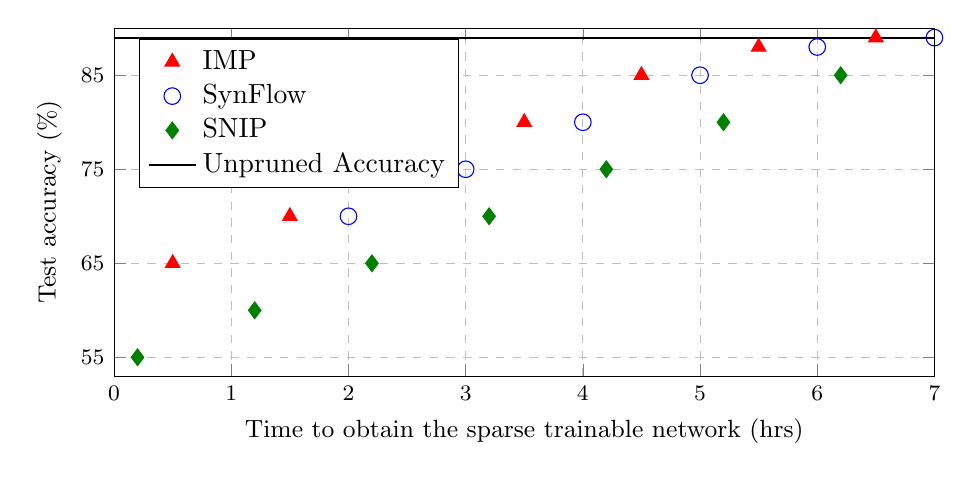
\begin{tikzpicture}
  \begin{axis}[
    width=12cm, height=6cm,
    xlabel={Time to obtain the sparse trainable network (hrs)},
    ylabel={Test accuracy (\%)},
    xmin=0, xmax=7,
    ymin=53, ymax=90,
    xtick={0,1,2,...,7},
    ytick={55,65,...,90},
    grid=both,
    grid style={dashed, gray!50},
    legend style={at={(0.03,0.97)}, anchor=north west},
    legend cell align={left},
    tick label style={font=\footnotesize},
    label style={font=\small},
  ]

    % IMP (Triangle markers)
    \addplot[impstyle] coordinates {
      (0.5, 65) (1.5, 70) (2.5, 75) (3.5, 80) (4.5, 85) (5.5, 88) (6.5, 89)
    };
    \addlegendentry{IMP}

    % SynFlow (Circle markers)
    \addplot[synflowstyle] coordinates {
      (2, 70) (3, 75) (4, 80) (5, 85) (6, 88) (7, 89)
    };
    \addlegendentry{SynFlow}

    % SNIP (Diamond markers)
    \addplot[snipstyle] coordinates {
      (0.2, 55) (1.2, 60) (2.2, 65) (3.2, 70) (4.2, 75) (5.2, 80) (6.2, 85)
    };
    \addlegendentry{SNIP}

    % Unpruned Accuracy (Solid black line)
    \addplot[unprunedstyle] coordinates {
      (0, 89) (7, 89)
    };
    \addlegendentry{Unpruned Accuracy}

  \end{axis}
\end{tikzpicture}

\end{document}